\documentclass{article}
\usepackage[french]{babel} 
\usepackage[utf8]{inputenc}
\usepackage{verbatim}
\usepackage{fullpage}
\usepackage{fancyhdr}
\usepackage{graphicx}
\usepackage{tikz}
\usepackage{fancyvrb}
\newcommand\userinput[1]{\textbf{#1}}
\usepackage{alltt}
\usepackage{xcolor}

%%% Les hyperliens %%%

%\pagestyle{fancy}
\renewcommand{\footrulewidth}{0.4pt}
\renewcommand{\headrulewidth}{0pt}
%\fancyhf{}
\lfoot{Girard Johan -- Odin Pierre}
\rfoot{ARC M1 INFO}


%%%% déclarations pour le titre %%%%

\author{\small \textsc{Girard Johan -- Odin Pierre}}


\title{
\includegraphics[width=2cm]{logo.jpg} \\ \vspace*{3cm} Techniques d’adaptation et de génie logiciel \\ 
 \vspace*{3mm} M1 Informatique \\ \vspace*{3cm} \hrule \vspace*{1cm} Compte rendu des TP\vspace*{1cm}  \hrule  \vspace*{5cm}} 



\date{\small \today}


%%%% Le Document %%%%

\begin{document}

\maketitle
\newpage

\section{Séance 1}

\subsection {Git}

Nous avons déjà utiliser git. Pas de problèmes.

\subsection {GitHub \& Travis-CI}

Notre dépôt : https://github.com/CCGIOD/tagl

Découverte de travis.

\subsection{Maven}

Découverte de Maven.

Création avec :
groupId: it
artifactId: cron4j-mvn
version: 2.5.5

\verb?mvn clean verify? marche et ajout de \verb?pushd cron4j-mvn && mvn clean verify && popd? dans .travis.yml

\subsection {Tests Unitaires avec JUnit 4}

\begin{alltt}
-------------------------------------------------------
 T E S T S
-------------------------------------------------------
Running it.sauronsoftware.SchedulingPatternTest
Tests run: 2, Failures: 1, Errors: 0, Skipped: 0, Time elapsed: 0.067 sec <<< FAILURE!
testPattern(it.sauronsoftware.SchedulingPatternTest)  Time elapsed: 0.011 sec  <<< FAILURE!
java.lang.AssertionError: 0 5 * *is correct
	at org.junit.Assert.fail(Assert.java:88)
	at org.junit.Assert.assertTrue(Assert.java:41)
	at it.sauronsoftware.SchedulingPatternTest.testPattern(SchedulingPatternTest.java:35)
	...

Results :

Failed tests:   testPattern(it.sauronsoftware.SchedulingPatternTest): 0 5 * *is correct

Tests run: 2, Failures: 1, Errors: 0, Skipped: 0
\end{alltt}

Correction : ajout d'une * : \verb?pattern="0 5 * * *";?

Ok dans travis

Nouveaux tests : 

\begin{alltt}
  @Test(expected = Exception.class)
  public void testCronParserFalse() throws Exception {
    TaskTable t = new TaskTable ();
    CronParser.parseLine(t,"chlagadeul");
  }

  @Test
  public void testCronParserTrue() throws Exception {
    TaskTable t = new TaskTable ();
    CronParser.parseLine(t,"0 5 * * * ls");
  }
\end{alltt}

Ok dans travis

\subsection {Git (suite)}

\begin{alltt}
<licenses>
    <!--Licence du projet-->
    <license>
      <name>GNU General Public License, version 3</name>
      <url>http://opensource.org/licenses/GPL-3.0</url>
    </license>
</licenses>
\end{alltt}

\subsection {Plugins}

Mais qu'est ce que la couverture de code ? En quoi c'est utile ?

La couverture de code est une technique qui permet de mesurer la quantité de code du programme qui est testé.
	     Cela sert donc à évaluer les tests. Si le taux de code testé est faible, cela veut dire que les tests sont mauvais
	     car il ne permettent pas de tester certaines parties du code qui pourraient contenir des erreurs ...

Pour les plugins voir la partie du pom.xml suivante :

\begin{alltt}
  <build>
    <plugins>
      <plugin>
	<groupId>org.apache.maven.plugins</groupId>
	<artifactId>maven-project-info-reports-plugin</artifactId>
	<version>2.7</version>
	<configuration>
	  <dependencyLocationsEnabled>false</dependencyLocationsEnabled>
	</configuration>
      </plugin>

      <plugin>
	<!-- Le plugin Cobertura est ajouté ici pour permettre d'éxécuter le goal cobertura pendant la phase package -->
	<groupId>org.codehaus.mojo</groupId>
	<artifactId>cobertura-maven-plugin</artifactId>
	<version>2.6</version>

	<!-- La couverture de code est une technique qui permet de mesurer la quantité de code du programme qui est testé.
	     Cela sert donc à évaluer les tests. Si le taux de code testé est faible, cela veut dire que les tests sont mauvais
	     car il ne permettent pas de tester certaines parties du code qui pourraient contenir des erreurs ... -->

	<configuration>
	  <formats>
	    <format>html</format> <!-- On sélectionne le format html -->
	  </formats>
	</configuration>
	<executions>
	  <execution>
	    <phase>package</phase>
	    <goals>
	      <goal>cobertura</goal>
	    </goals>
	  </execution>
	</executions>
      </plugin>
    </plugins>
  </build>

  <!-- Utiliser 'mvn site' -->
  <reporting>
    <plugins>

      <!-- Ajout de la couverture de code sur le site -->
      <!-- Le plugin Cobertura est ajouté ici pour qu'il apparaisse sur le site -->
      <plugin>
	<groupId>org.codehaus.mojo</groupId>
	<artifactId>cobertura-maven-plugin</artifactId>
	<version>2.6</version>
	<configuration>
	  <formats>
	    <format>html</format>
	  </formats>
	</configuration>
      </plugin>

      <!-- Ajout de la javadoc sur le site -->
      <plugin>
	<groupId>org.apache.maven.plugins</groupId>
	<artifactId>maven-javadoc-plugin</artifactId>
	<version>2.9.1</version>
      </plugin>

      <!-- Ajout du résultat des tests unitaires sur le site -->
      <plugin>
	<groupId>org.apache.maven.plugins</groupId>
	<artifactId>maven-surefire-report-plugin</artifactId>
	<version>2.4.3</version>
      </plugin>

      <!-- Ajout du taglist sur le site -->
      <plugin>
        <groupId>org.codehaus.mojo</groupId>
        <artifactId>taglist-maven-plugin</artifactId>
        <version>2.4</version>
         <configuration>
          <tagListOptions>
            <tagClasses>
              <tagClass>
                <displayName>Todo Work</displayName>
                <tags>
                  <tag>
                    <matchString>todo</matchString>
                    <matchType>ignoreCase</matchType>
                  </tag>
                  <tag>
                    <matchString>FIXME</matchString>
                    <matchType>exact</matchType>
                  </tag>
                </tags>
              </tagClass>
            </tagClasses>
          </tagListOptions>
        </configuration>
      </plugin>

      <!-- Ajout de la visualisation des sources sur le site -->
      <plugin>
	<groupId>org.apache.maven.plugins</groupId>
	<artifactId>maven-jxr-plugin</artifactId>
	<version>2.4</version>
      </plugin>

      <!-- D'autres plugins pourraient être ajoutés ci-après ... -->
      
    </plugins>
  </reporting>
\end{alltt}

En faisant mvn site on obtient le site qui contient bien les rapports :


\begin{center}
\frame{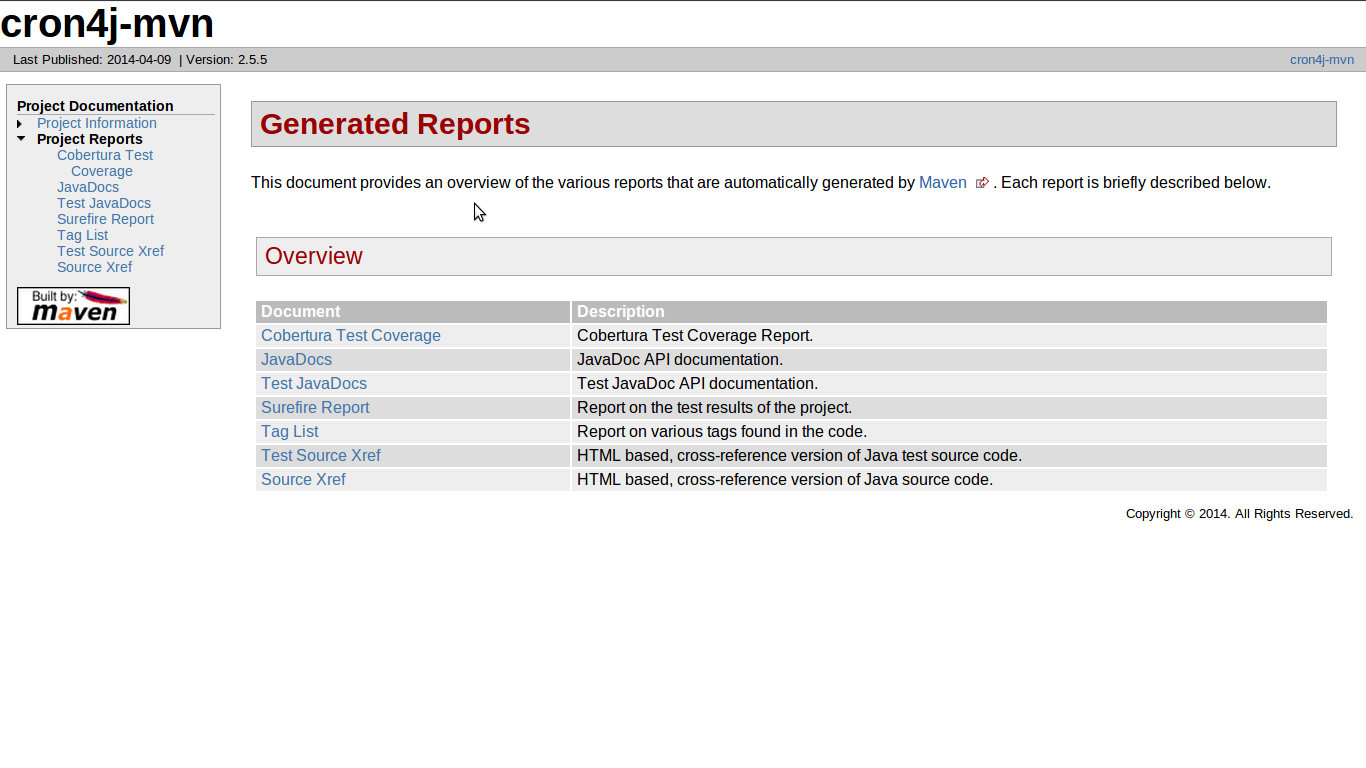
\includegraphics[width=15cm]{screen_report}}
\end{center}

\section{Séance 2: AOP \& AspectJ}

On ajoute les dépendances :
\begin{alltt}
  <dependencies>
<dependency>
      <groupId>org.aspectj</groupId>
      <artifactId>aspectjrt</artifactId>
      <version>1.7.4</version>
    </dependency>
    <dependency>

      <groupId>org.aspectj</groupId>
      <artifactId>aspectjweaver</artifactId>
      <version>1.7.4</version>
    </dependency>

    <dependency>
      <groupId>org.aspectj</groupId>
      <artifactId>aspectjtools</artifactId>
      <version>1.7.4</version>
    </dependency>
  </dependencies>
\end{alltt}
Et : 

\begin{alltt}
  <pluginManagement>
    <plugins>
      <plugin>
	<groupId>org.codehaus.mojo</groupId>
	<artifactId>aspectj-maven-plugin</artifactId>
	<version>1.6</version>
	<configuration>
	  <complianceLevel>1.6</complianceLevel>
	  <outxml>true</outxml>
	  <verbose>true</verbose>
	  <showWeaveInfo>true</showWeaveInfo>
	</configuration>
	<executions>
	  <execution>
	    <goals>
	      <goal>compile</goal>
	      <goal>test-compile</goal>
	    </goals>
	  </execution>
	</executions>
      </plugin>
    </plugins>
  </pluginManagement>
\end{alltt}

et :

\begin{alltt}
<plugin>
	<groupId>org.codehaus.mojo</groupId>
	<artifactId>aspectj-maven-plugin</artifactId>
      </plugin>
\end{alltt}

On a une erreur a cause de Corbertura en même temps que aspectj donc on a enlevé Corbertura executé pendant la phase package!

On ajoute la classe :

\begin{alltt}

package it.sauronsoftware.cron4j;

import org.aspectj.lang.annotation.Aspect;
import org.aspectj.lang.annotation.Before;
import org.aspectj.lang.annotation.After;

@Aspect
    public class AspectTraceRun {

    @Before("execution(* RunnableTask.execute(..))")
	public void printB () { 
	System.out.println("run() is starting!");
    }

    @After("execution(* RunnableTask.execute(..))")
	public void printA () { 
	System.out.println("run() is ending!");
    }
}
\end{alltt}

Le test :

\begin{alltt}
@Test
	public void testRunableTask() {
	Task task = new RunnableTask(new HelloRunnable());
	Scheduler scheduler = new Scheduler();
	scheduler.schedule("* * * * *", task);
	scheduler.start();
	try {
	    Thread.sleep(1L * 60L * 1000L);
	} catch (InterruptedException e) {}
	scheduler.stop();
    }
\end{alltt}

\subsection{ThreadLocal}

Ajout d'une couple COupleInteger pour gérer un id et un compteur.

\begin{alltt}
@Aspect
    public class AspectTraceRun {

    private static final AtomicInteger nextId = new AtomicInteger(0);

    public static class CoupleInteger {
     	private Integer id;
	private Integer cpt;
	
	public CoupleInteger (){ this.id=nextId.getAndIncrement(); this.cpt=0;}
	
	public Integer getId () { return id; }
	public Integer getCpt () { return cpt; }
        public void incr () { cpt++; }
    }

    private static final ThreadLocal<CoupleInteger> threadId =
	new ThreadLocal<CoupleInteger>() {
	@Override protected CoupleInteger initialValue() {
	    return new CoupleInteger();
	}
    };

    public static CoupleInteger get() {
	return threadId.get();
    }

    @Before("execution(* RunnableTask.execute(..))")
	public void printB () { 
        threadId.get().incr();
	System.out.println("run() is starting! (ThreadLocal: id:"+get().getId()+" cpt: "+get().getCpt()+")");
    }

    @After("execution(* RunnableTask.execute(..))")
	public void printA () { 
	System.out.println("run() is ending!");
    }
}
\end{alltt}

Ce qui donne : 

\begin{alltt}

-------------------------------------------------------
 T E S T S
-------------------------------------------------------
Running it.sauronsoftware.SchedulingPatternTest
Tests run: 4, Failures: 0, Errors: 0, Skipped: 0, Time elapsed: 0.062 sec
Running it.sauronsoftware.SchedulingAjTest
run() is starting! (ThreadLocal: id:0 cpt: 1)
Hello from a thread (1)
run() is ending!
run() is starting! (ThreadLocal: id:1 cpt: 1)
Hello from a thread (2)
run() is ending!
run() is starting! (ThreadLocal: id:2 cpt: 1)
Hello from a thread (3)
run() is ending!
Tests run: 1, Failures: 0, Errors: 0, Skipped: 0, Time elapsed: 179.999 sec

Results :

Tests run: 5, Failures: 0, Errors: 0, Skipped: 0
\end{alltt}

\section{TP 3}

\section{TP 4}



\end{document}

